\documentclass{standalone}
\usepackage{tikz}
\usepackage{pgfplots}
\usepackage{nono}
\begin{document}
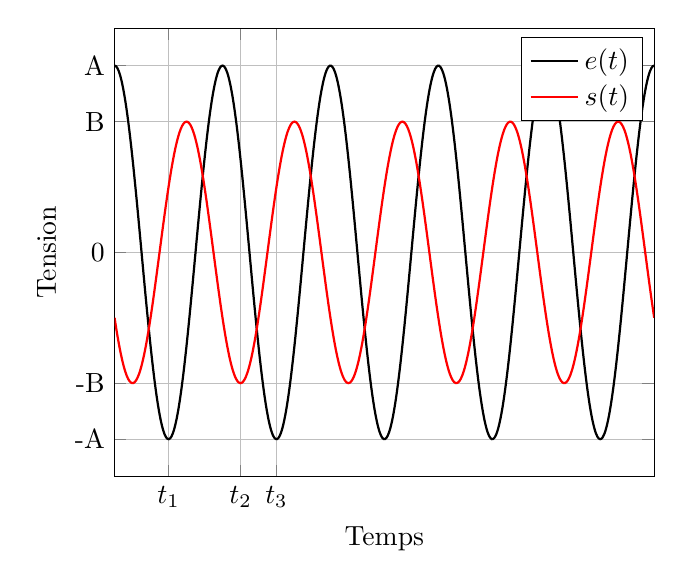
\begin{tikzpicture} 
  \begin{axis}[
    grid=both,
    xmin=0,xmax = 5*360,
    xtick={180, 420,540},
    xticklabels={$t_1$, $t_2$, $t_3$},
    ytick={-1, -0.7, 0, 0.7, 1},
    yticklabels={-A, -B, 0, B, A},
    xlabel=Temps,
    ylabel=Tension,
    ]
  \addplot[smooth, domain=0:360*5, samples=400, thick]{cos(x)};
  \addlegendentry{$e(t)$}; 
  \addplot[smooth, domain=0:360*5, samples=400, thick, red]{0.7*cos(x+120)};
  \addlegendentry{$s(t)$}; 
  \end{axis}
\end{tikzpicture}
\end{document}
